\section{Graphen}
	\begin{definition}[Ungerichteter Graph]
		Ein \textbf{ungerichteter Graph} $G$ ist ein Tripel $(V, E, \Psi)$, für das
		\begin{enumerate}
			\item $V$ und $E$ endliche Mengen sind und
			\begin{itemize}
				\item $V$ ist die Knotenmenge
				\item $E$ ist die Kantenmenge
			\end{itemize}
			\item $\Psi$ eine Funktion mit
			\begin{equation*}
				\Psi : E \to \set{X \subseteq V \vert 1 \le \card{X} \le 2}
			\end{equation*}
			ist.\\
		\end{enumerate}
		\begin{itemize}
				\item Zwei Kanten $e, e'$ sind \textbf{parallel}, wenn $\Psi(e) = \Psi(e')$.
				\item Eine Kante $e$ ist eine \textbf{Schleife}, falls $\card{\Psi(e)} = 1$.
				\item Ein Graph ohne parallele Kanten und Schleifen heißt \textbf{einfach}. Man schreibt dann $G = (V, E)$ mit $E(G)$ der Kantenmenge von G.
				\begin{itemize}[label=$\hookrightarrow$]
					\item  In einem einfachen Graphen kann man $\set{v_i, v_j}$ für eine Kante $e_{i,j}$ zwischen $v_i$ und $v_j$ schreiben.
				\end{itemize}
				\item $\card{E}$ ist die Zahl der Kanten und $\card{V}$ die Zahl der Knoten von $G$.
				\begin{itemize}[label=$\hookrightarrow$]
					\item Oft verwendet man $n$ für $\card{V}$ und $m$ für $\card{E}$.
				\end{itemize}
			\end{itemize}
	\end{definition}
	\begin{figure}[ht]
			\begin{subfigure}[c]{0.5\textwidth}
				\begin{center}
				\begin{tikzpicture}
					\node[circle, fill, black, scale = .8] (A) {};
					\node[circle, fill, black, scale = .8, above = 1cm of A] (B) {};
					\path (A) edge[bend right] (B);
					\path (A) edge[bend left] (B);
				\end{tikzpicture}
				\end{center}
				\subcaption{parallele Kanten}
			\end{subfigure}
			\begin{subfigure}[c]{0.5\textwidth}
				\begin{center}
				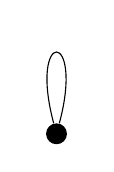
\begin{tikzpicture}[every loop/.style={}]
					\node[circle, fill, black, scale = .8] (A) {};
					\path[every node/.style={font=\sffamily\small}] (A) edge[loop above, scale = 2.5] (A);
				\end{tikzpicture}
				\end{center}
				\subcaption{Schleife}
			\end{subfigure}
	\end{figure}
	\begin{definition}[Nachbarschaft in Graphen]
		Eine Kante $e = \set{v, w}$ in einem Graphen verbindet zwei Knoten $v$ und $w$. Der Knoten $v$ ist dann Nachbar von $w$, d.h. $v$ und $w$ sind \textbf{adjazent} (\dq benachbart\dq). Außerdem ist sowohl $v$ als auch $w$ \textbf{inzident} (\dq zusammentreffend mit\dq) zu $e$.
	\end{definition}
	\begin{definition}[Knotengrad]
		Der \textbf{Grad} eines Knotens $v$ ist die Anzahl der inzidenten Kanten und wird bezeichnet mit $deg(v)$ (auch $\delta(v)$).\\[5pt]
		Ein Knoten $v$ heißt \textbf{isoliert}, wenn $deg(v) = 0$.
	\end{definition}
	\begin{satz}
		Sei $G = (V, E)$ ein Graph. Dann gilt
		\begin{equation*}
			\sum_{v \in V} deg(v) = 2\card{E}.
		\end{equation*}
		D.h. die Summe über alle Knotengrade ist gleich 2-mal die Anzahl der Kanten.
	\end{satz}
	\begin{lemma}[Handshake-Lemma]
		In jedem Graphen ist die Anzahl der Knoten mit ungeradem Grad gerade.
	\end{lemma}
	\begin{definition}[Teilgraph]
		Ein Teilgraph $H = (V(H), E(H))$ eines Graphen $G =\\ (V(G), E(G))$ ist ein Graph mit
		\begin{eqnarray*}
			V(H) &\subseteq& V(G),\\
			E(H) &\subseteq& E(G).
		\end{eqnarray*}
		$H$ ist \textbf{aufspannend}, wenn $V(H) = V(G)$ gilt.
	\end{definition}
	\begin{definition}[Isomorph]
		Seien $G = (V(G), E(G))$ und $H = (V(H), E(H))$ zwei Graphen. Wenn es eine bijektive Abbildung $f : V(G) \to V(H)$ gibt, sodass $\set{v, w} \in E(G)$ gilt, genau dann, wenn $\set{f(v), f(w)} \in E(H)$ gilt, dann nennen wir die Graphen \textbf{äquivalent} (oder \textbf{isomorph}).
	\end{definition}
	
	\subsection{Datenstrukturen für Graphen}
	\begin{definition}[Adjazenzmatrix]
		Eine \textbf{Adjazenzmatrix} $A = (a_{vw})$ eines Graphen $G = (V, E)$ beschreibt, welche Knoten $v_i$ zu welchen Knoten $v_j$ adjazent sind ($v_i, v_j \in V$). Die Matrix hat die Dimension $n\times n$, wobei $n = \card{V}$.\\
		Es gilt $A\in \set{0, 1}^{n\times n}$ mit
		\begin{equation*}
			a_{vw} := \begin{cases*}
				1 \text{ für } \set{v,w} \in E\\
				0 \text{ sonst}
			\end{cases*}
		\end{equation*}
		Eine Adjazenzmatrix ist quadratisch und symmetrisch. Für einfache Graphen enthält die Diagonale ausschließlich Nullen.\\
	\end{definition}
	\begin{definition}[Inzidenzmatrix]
		Eine \textbf{Inzidenzmatrix} $A = (a_{ve})$ eines Graphen $G = (V, E)$ beschreibt, welche Knoten $v_i \in V$ zu welchen Kanten $e_j \in E$ inzident sind. Die Matrix hat die Dimension $n\times m$, wobei $n = \card{V}$ und $m = \card{E}$.\\
		Es gilt $A\in \set{0, 1}^{n\times m}$ mit
		\begin{equation*}
			a_{ve} := \begin{cases*}
			1 \text{ für } v \in e\\
			0 \text{ sonst}
			\end{cases*}
		\end{equation*}
		Für große Graphen enthält die Matrix tendenziell viele Nullen.
	\end{definition}
	\begin{definition}[Kantenliste]
		Eine \textbf{Kantenliste} eines Graphen $G = (V, E)$ ist eine Liste aus zweielementigen Knotenmengen $\set{v_i, v_j} \in E$, die eine Kante von $v_i$ zu $v_j$ beschreiben $(v_i, v_j \in V)$.\\ Die Kantenliste benötigt $\Theta(m~log(n))$ Speicherplatz und ist damit sparsamer als die Inzidenzmatrix (für $n \ge 8$).
	\end{definition}
	\begin{definition}[Adjazenzliste]
		Eine \textbf{Adjazenzliste} eines Graphen $G = (V, E)$ gibt zu jedem Knoten $v_i$ die benachbarten Knoten $v_j$ an $(v_i, v_j \in V)$.\\
		Das ist etwas praktischer als die Kantenliste, wenn man für Graphenalgorithmen direkten Zugriff auf die Nachbarn eines Knotens benötigt. Man muss nicht die Nachbarn erst mühsam aus einer Liste heraussuchen.\\
		Die Adjazenzliste benötigt $\Theta(n~log(n)+m~log(n))$ Speicherplatz. Im Allgemeinen sind Graphen mit vielen isolierten Knoten (ohne Kanten) uninteressant, d.h z.B. $m\ge \frac{n}{2}$ oder $m\ge n$ o.ä. Also wieder $\Theta(m~log(n))$.
	\end{definition}
	
	\subsection{Wege und Pfade}
	\begin{definition}[Kantenfolge]
		Eine \textbf{Kantenfolge} $W$ in einem Graphen $G = (V, E)$ ist eine Folge $v_1, e_1, v_2, e_2, v_3, ..., e_k, v_{k+1}$ mit $k \ge 0,~e_i = \set{v_i, v_{i+1}} \in E$
	\end{definition}
	\begin{figure}[ht]
		\begin{center}
			\begin{tikzpicture}
			\node[circle, fill, black, scale = .8] (A) {};
			\node[circle, fill, black, scale = .8, above = 1cm of A] (B) {};
			\node[circle, fill, black, scale = .8, left = 1cm of A] (C) {};
			\node[circle, fill, black, scale = .8, right = 1cm of B] (D) {};
			\node[circle, fill, black, scale = .8, below = 1cm of D] (E) {};
			\node[circle, fill, black, scale = .8, right = 1cm of E] (F) {};
			\path (A) edge[red] (B);
			\path (A) edge[red] (C);
			\path (C) edge (B);
			\path (B) edge[red] (D);
			\path (A) edge (D);
			\path (A) edge (E);
			\path (E) edge (F);
			\path (D) edge[red] (F);
			\end{tikzpicture}
		\end{center}
		\caption{Kantenfolge in $G$}
	\end{figure}
	\begin{definition}[Weg]
		Wiederholt sich keine Kante in einer Kantenfolge, dann spricht man von einem \textbf{Weg}. Ein \textbf{geschlossener Weg} (auch Tour) kehrt am Ende zum Startknoten zurück. Ein \textbf{Eulerweg} benutzt alle Kanten eines Graphen. Eine \textbf{Eulertour} kehrt außerdem zum Startknoten zurück.
	\end{definition}
	\begin{definition}[Pfad]
		Wiederholt sich kein Knoten in einer Kantenfolge, dann sprichtman von einem \textbf{Pfad}. Ein \textbf{Kreis} ist ein geschlossener Pfad, d.h. der Pfad kehrt zum Startknoten zurück. Ein \textbf{Hamiltonpfad} besucht alle Knoten eines Graphen. Ein \textbf{Hamiltonkreis} (auch Hamiltontour) kehrt außerdem zum Startknoten zurück.
	\end{definition}
	\begin{satz}
		Sei $G$ ein Graph mit Adjazenzmatrix $A$. Der Koeffizient $a_{vw}^{(m)}$ von $A^m$ gibt die Anzahl der Kantenfolgen der Länge $m$ von Knoten $v$ zu Knoten $w$ an. Insbesondere gilt $a_{vv}^{(2)} = deg(v)$.
	\end{satz}
	\begin{definition}[Zusammenhängend]
		Ein Graph $G$ heißt \textbf{zusammenhängend}, wenn es zwischen je zwei Knoten aus $G$ einen Weg gibt.\\[5pt]
		Ein maximaler zusammenhängender Teilgraph von $G$ heißt eine \textbf{(Zusammenhangs-) Komponente} von $G$.
	\end{definition}
	\begin{figure}[ht]
	\begin{center}
		\begin{tikzpicture}
			\node[circle, fill, black, scale = .8] (A) {};
			\node[circle, fill, black, scale = .8, above = 1cm of A] (B) {};
			\node[circle, fill, black, scale = .8, left = 1cm of A] (C) {};
			\node[circle, fill, black, scale = .8, right = 2.5cm of B] (D) {};
			\node[circle, fill, black, scale = .8, below right = 1cm of D] (E) {};
			\node[circle, fill, black, scale = .8, below left = 1cm of D] (F) {};
			\node[circle, fill, black, scale = .8, right = 3cm of D] (G) {};
			\node[circle, fill, black, scale = .8, below right = 1cm of G] (H) {};
			\node[circle, fill, black, scale = .8, below left = 1cm of G] (I) {};
			\node[circle, fill, black, scale = .8, below left = 1cm of H] (J) {};
			\path (A) edge (B);
			\path (A) edge (C);
			\path (C) edge (B);
			\path (D) edge (F);
			\path (D) edge (E);
			\path (G) edge (H);
			\path (G) edge (I);
			\path (H) edge (J);
			\path (I) edge (J);
		\end{tikzpicture}
		\caption{Graph mit 3 Zusammenhangskomponenten}
	\end{center}
	\vspace*{-15pt}
	\end{figure}
	\begin{satz}[notwendiges Kriterium]
		Ein zusammenhängender Graph $G$ mit $n$ Knoten muss zumindest $n - 1$ Kanten haben.
	\end{satz}
	\begin{satz}[hinreichendes Kriterium]
		Ein Graph $G$ mit mehr als $\frac{(n-1)(n-2)}{2}$ Kanten ist zusammenhängend.
	\end{satz}
	\begin{problem}[Zusammenhang]~\\[5pt]
		\hspace*{10pt}\textbf{Gegeben: } Ein Graph $G = (V, E)$.\\[5pt]
		\hspace*{10pt}\textbf{Gesucht: } Ist $G$ zusammenhängend?
	\end{problem}
	\begin{algorithm}[H]
		\Input{Graph $G$}
		\Output{Ist $G$ zusammenhängend}\vspace*{5pt}
		Markiere einen beliebigen Startknoten.\\
		Für jeden im voherigen Schritt markierten Knoten: Markiere alle noch nicht markierten adjazente Knoten. Wurde kein neuer Knoten markiert, dann 3. Sonst wiederhole 2.\\
		Sind noch unmarkierte Knoten übrig \Return \dq $G$ ist nicht zusammenhängend\dq. Sonst \dq$G$ ist zusammenhängend\dq.
		\caption{Algorithmus zum Entscheiden ob ein Graph $G$ zusammenhängend ist. Laufzeit: $O(\card{E})$}
	\end{algorithm}
	\begin{satz}
		Ein Graph $G$ mit Adjazenzmatrix $A$ ist zusammenhängend, genau dann, wenn
		\begin{equation*}
			Z = I_n + A + A^2 + ... + A^{n-1} \text{ mit } z_{vw} \neq 0~ \forall v, w \in \set{1, ..., n}
		\end{equation*}
		existiert.
	\end{satz}

	\subsection{Eulerwege und Hamiltonpfade}
	\begin{problem}[Eulerweg]~\\[5pt]
		\hspace*{10pt}\textbf{Gegeben: } Ein Graph $G = (V, E)$.\\[5pt]
		\hspace*{10pt}\textbf{Gesucht: } Ein Eulerweg $W$ in $G$ -  oder ein Argument, dass kein Eulerweg existiert.
	\end{problem}
	\begin{satz}
		Ein Graph $G = (V, E)$ besitzt genau dann einen Eulerweg, wenn es höchstens zwei Knoten mit ungeradem Grad gibt.
	\end{satz}
	\begin{algorithm}
		\Input{Graph $G$}
		\Output{Ein Weg in $G$}\vspace*{5pt}
		Starte in einem Knoten $v_0$ \newline(wenn einer mit ungeradem Grad existiert, dort, sonst beliebig)\\
		$i \leftarrow 0$\\
		\While{es gibt eine zu $v_i$ inzidente Kante}
		{wähle eine zu $v_i$ inzidente, unbenutze Kante $\set{v_i, v_j}$\\
		laufe zum Nachbarknoten $v_j$\\
		lösche $\set{v_i, v_j}$ aus der Menge der unbenutzen Kanten\\
		$v_{i+1} \leftarrow v_j$\\
		$i \leftarrow i+1$
		}
		\caption{Algorithmus zum Finden eines Weges in einem Graphen}
	\end{algorithm}
	\begin{satz}
		Wenn der Algorithmus 2 stoppt, bleibt ein eulerscher Graph zurück, d.h. ein Graph mit lauter Knoten geraden Grades.
	\end{satz}
	\begin{korollar}~
		\begin{enumerate}
			\item Zwei geschlossene Wege mit einem gemeinsamen Knoten kann man in einen geschlossenen Weg verwandeln.
			\item Man kann aus allen Wegen einen Weg machen, wenn der Graph zusammenhängend ist, indem man immer wieder 1. anwendet.
		\end{enumerate}
	\end{korollar}
	\begin{algorithm}
		\Input{Zusammenhängender Graph $G$ mit höchstens 2 ungeraden Knoten}
		\Output{Ein Eulerweg, bzw. eine Eulertour in $G$}\vspace*{5pt}
		Starte in einem Knoten $v$ \newline(wenn einer mit ungeradem Grad existiert, dort, sonst beliebig)\\
		verwende Algorithmus 2, um einen Weg $W$ von $v$ aus zu bestimmen\\
		\While{es existieren unbenutzte Kanten}
		{wähle einen Knoten $w$ aus $W$ mit positivem Grad im Restgraphen\\
		verwende Algorithmus 2, um einen Weg $W'$ von $w$ aus zu bestimmen\\
		verschmelze $W$ und $W'$\\
		}
		\caption{Algorithmus zum Finden eines Eulerweges oder einer Eulertour}
		\label{fig:Algorithmus}
	\end{algorithm}
	\begin{algorithm}[H]
		\Input{Zusammenhängender Graph $G$ mit höchstens 2 ungeraden Knoten}
		\Output{Ein Eulerweg, bzw. eine Eulertour in $G$}\vspace*{5pt}
		Starte in einem Knoten $v_0$ \newline(wenn einer mit ungeradem Grad existiert, dort, sonst beliebig)\\
		$i \leftarrow 0$\\
		\While{es gibt eine zu $v_i$ inzidente, unbenutzte Kante}
		{wähle eine dieser Kanten $\set{v_i, v_j}$, die den Restgraph zshgd. lässt\\
		laufe zum Nachbarknoten $v_j$\\
		markiere $\set{v_i, v_j}$ als benutzt\\
		$v_{i+1} \leftarrow v_j$\\
		$i \leftarrow i+1$
		}
		\caption{Algorithmus von Fleury zum Finden eines Eulerweges oder einer Eulertour}
	\end{algorithm}
	\begin{satz}[hinreichendes Kriterium]
		Wenn ein Graph mit $n$ Knoten mindestens $\frac{1}{2}(n-1)(n-2)+2$ Kanten hat, dann besitzt er einen Hamiltonkreis.
	\end{satz}
